\chapter{Hydrogen}
\label{chap:h2}
    \section{Motivation}
        Hydrogen is an extremely important ingredient in many industries including fertilizers, petroleum, aerospace as rocket fuel and energy as an alternative fuel source \cite{Jacobsen2007}. Additionally, the properties of mixtures of hydrogen and other gases are also important in several other fields ranging from metrology (H$_{\rm 2}$ + H$_{\rm 2}$O) \cite{Hodges2004} to astrophysics (H$_{\rm 2}$ + He) \cite{Boothroyd2002,Boothroyd2003} to superfluidics \cite{Patkowski2008,Grebenev2000}. Therefore, computing really precise and accurate physical properties of hydrogen is vital to several industries as well as research institutions.

        Historically, hydrogen has been, and still is, one of the most studied compounds in quantum chemistry owing to its extremely simple electronic structure comprising just one electron. Molecular hydrogen exists in two forms with significantly different physical properties \cite{Jacobsen2007}: 1) parahydrogen with anti-parallel nuclear spins and 2) orthohydrogen with parallel nuclear spins. Hydrogen also has two isotopes Deuterium (D) and Tritium (T) with 1 and 2 neutrons respectively. Several studies \cite{Goodwin1963,Kolos1986,Schwenke1988,Mielke2002,Manzhos2010,Garberoglio2010,Garberoglio2012,Sakoda2012,Garberoglio2013,Garberoglio2014} (both computational as well as experimental) of different combinations of the hydrogen molecule and its isotopes ($\allowbreak {\rm H_2, H_3, (H_2)_2, (H_2)_3, HD, HT, D_2, T_2}$ etc.) have been performed to gain further insight into the nature of interactions of these systems. However, for the purpose of evaluating fully quantum virial coefficients using \abinitio{} potentials, we restrict our attention primarily to the hydrogen dimer ${\rm (H_2)_2}$ and consider both the rigid as well as flexible monomer cases.

    \section{Recent Developments}
        In this section, we give an overview of some the \abinitio{} \PESs{} that have been developed for studying the hydrogen dimer and in the interest of brevity, we restrict our discussion to the \PESs{} that were developed on or after the year 2000.\\

        Diep and Johnson's \cite{Diep2000} pioneering work lead not only to the development of the PIMC method but also two \abinitio{} \PESs{} for the dimer with rigid monomers. One using the vibrationally-averaged bond length of the dimer and another using a slightly smaller equilibrium value, in order to study the effect of bond lengths on the \PESs{}. Thirty seven unique angular configurations were used in the construction of these \PESs{} (and their corresponding spherical harmonics fits) and electron correlation effects were accounted at the MP2, MP3, MP4 and CCDS(T) levels of theory. They observed excellent agreement of their calculated second virial coefficient values with experiments for T = 15 to 500K. They also concluded that the differences observed in the \PESs{} based on different bond lengths were small. Boothroyd et al. \cite{Boothroyd2002} reported a rigid monomer PES (Ad) that was fit to \Sim{} 48 000 \abinitio{} energies out of which \Sim{} 42 000 were computed using the MRD-CI program of Buenker and Peyerimhoff \cite{Buenker1974}. They observed significant improvement over previous \PESs{} in terms of its rms error. Robert J. Hinde \cite{Hinde2008} reported a six dimensional PES that included monomer flexibility as well and used it for studying the IR and Raman transition energies. Patkowski et al. \cite{Patkowski2008} reported a rigid monomer PES that was computed at the CCSD(T) level of theory using very large orbital basis sets. They reported second virial coefficients that were in better agreement with experiments than previous \PESs{}. It was also found that including quantum effects becomes important at \Sim{} 200K for PIMC calculations of virial coefficients. Most recently, Van and Deiters \cite{Tat2015} have reported a new \abinitio{} PES at the CCSD(T) level of theory and observed very good agreement of their calculated virial coefficients with experimental results (where available).

    \section{Computational details}
    \label{sec:Computational details}

        We performed calculations for three different models of H$_2$, differing primarily in their treatment of the intramolecular bond:

        Model 1 : We use the rigid inter-molecular potential due to Patkowski et al.\cite{Patkowski2008} (denoted as V$_{pat}$), with the H-H bond length fixed at all temperatures to the ground state value $r_0 ( = $1.448736 bohrs, same as in \cite{Patkowski2008}). Due to nonphysical energies returned by V$_{pat}$ at small inter-molecular separations, an artificial spherical hard core (with a diameter $d = 1${\AA}) is used.

        Model 2 : We use the flexible inter-molecular potential due to Garberoglio et al.\cite{Garberoglio2012} (denoted as V$_{hp}$), with a fixed but temperature-dependent H-H bond length, computed at each temperature to its average value $\left< r \right>_T$ (see Ref. \cite{Garberoglio2012} for details). For V$_{hp}$, instead of an artificial spherical hard core, the potential is calculated with an inter-molecular distance $R$ which is the larger of ($R,\: 1.4${\AA}) and a bond length $b$ which is the smaller of ($b,\: 1.2${\AA}).

        Model 3 : We use V$_{hp}$ and allow the bond length value to vary during the calculation. The intra-molecular potential that we use is due to Mielke et al.\cite{Mielke2002} who fitted the data of Kolos et al.\cite{Kolos1986} to obtain a ground state potential.

        Mayer sampling Monte Carlo was used to sample the intermolecular distance, while the direct methods described above were used to sample path-integral image position, orientations and (where appropriate) bond lengths. These different MC moves were chosen with equal probability within each simulation. We ran simulations at 33 temperatures going from $T =$ 15 K $\to$ 2000 K to compare our results for the three models against Garberoglio et al.\cite{Garberoglio2014}. We ran additional simulations at 53 temperatures going from $T =$ 16 K $\to$ 423.15 K for which experimental $B_2$ values were reported in Goodwin et al.\cite{Goodwin1963}. Although the $B_2$ values in \cite{Garberoglio2014} were calculated after choosing $P$ as a function of $T$, we ran calculations for $P = 8, 16, 32$ and $64$ for all temperatures considered because we wanted to assess the performance of the algorithms. For each value of $P$, we used a total of $10^7$ samples to evaluate the virial coefficient using the MSMC\cite{Singh2004} method. We divide the $10^7$ samples into $10^4$ blocks of $10^3$ samples each and compute block averages for the different quantities prescribed by MSMC. Using the $10^4$ block-averages, we calculate the overall averages and their standard error, and use error propagation formulas to arrive at the final uncertainties (reported here) of the virial coefficients. A reference hard sphere diameter of 3{\AA} was used for all simulations.

        Note that all simulations performed for the conditions mentioned above, were to compute the Boltzmann contribution to the virial coefficient using only Boltzmann-type configuration samples. Additionally, we also performed simulations, for each of the cases mentioned above, to compute the exchange contribution to the virial coefficient using only exchange-type configuration samples. We combine the two contributions according to their ratio as given in Fig. 2 of Garberoglio et al. \cite{Garberoglio2014} to compute the final virial coefficient values reported here. Since the ratio was zero for $T > 225$K, suggesting that exchange contributions were negligible at higher temperatures, we evaluated the exchange contributions only for temperatures $T \le 225$K. In addition, we ran simulations for $P = 128$ for $T \le 100$K and $P = 256$ for $T = 15K, 20$K for the Boltzmann as well as exchange cases for Model 3.

    \section{Results and discussion}
    \label{sec:Results and discussion}
        Presented below are the results of our calculation of the virial coefficients of \emph{para}-H$_2$ as a function of temperature. Garberoglio et al.\cite{Garberoglio2014} previously reported second virial coefficients using VEGAS\cite{Lepage1972} algorithm for the three models explained in the previous section, and this provides a suitable reference set of data for comparison. For other literature values and/or experimental data, the interested reader may see references\cite{Goodwin1963, Patkowski2008, Leachman2009, Sakoda2012, Garberoglio2012, Garberoglio2014}). Henceforth, by ``reference values", we mean the values reported in \cite{Garberoglio2014} under similar conditions. All virial coefficient and other relevant values are tabulated at the end of this chapter.

        We also examine the performance in terms of percentage of moves accepted for both the orientation and the bond length algorithms, considered as a function of temperature for the different simulation options mentioned above.

        \subsection{Rigid-bond models -- Orientation trials}
            In this section we examine the results for Models 1 and 2, which are the rigid-bond models, by which we scrutinize the validity and performance of the orientation-sampling trial, by itself. We begin by noting that the number of images used by Garberoglio for achieving converged results \cite{Patkowski2008} for Model 1 was calculated as:
            \begin{equation}
            \label{eq:s1P}
                P = 3600 \textrm{K}/T
            \end{equation}
According to Eq. \eqref{eq:s1P} the temperature at which we require $P > 64$ to achieve converged results for Model 1 is 50 K. We also note that we have used a maximum of $P = 64$ images for all temperatures. Therefore we expect to see significant differences between our virial coefficient values for Model 1 and the corresponding reference values for $T \le 50 $K.

            Similarly, we have for Model 2 \cite{Garberoglio2012}:
            \begin{equation}
            \label{eq:s2P}
                P = \lceil 2500 \textrm{K}/T + 7 \rceil
            \end{equation}
            where $\lceil x \rceil$ denotes the smallest integer larger than $x$.
According to Eq. \eqref{eq:s2P} the temperature at which we require $P > 64$ to achieve converged results for Model 2 is 40 K. Therefore we expect to see significant differences between our virial coefficient values for Model 2 and the corresponding reference values for $T \le 40 $K. Although for a given temperature $T$, Eqs. \eqref{eq:s1P} and \eqref{eq:s2P} provide a good estimate of $P$ required for achieving converged results, in practice, one might be able to achieve convergence with fewer $P$ as well.

            \subsubsection{$B_2$ values}
                \begin{figure}[!htbp]
                    \centering
                    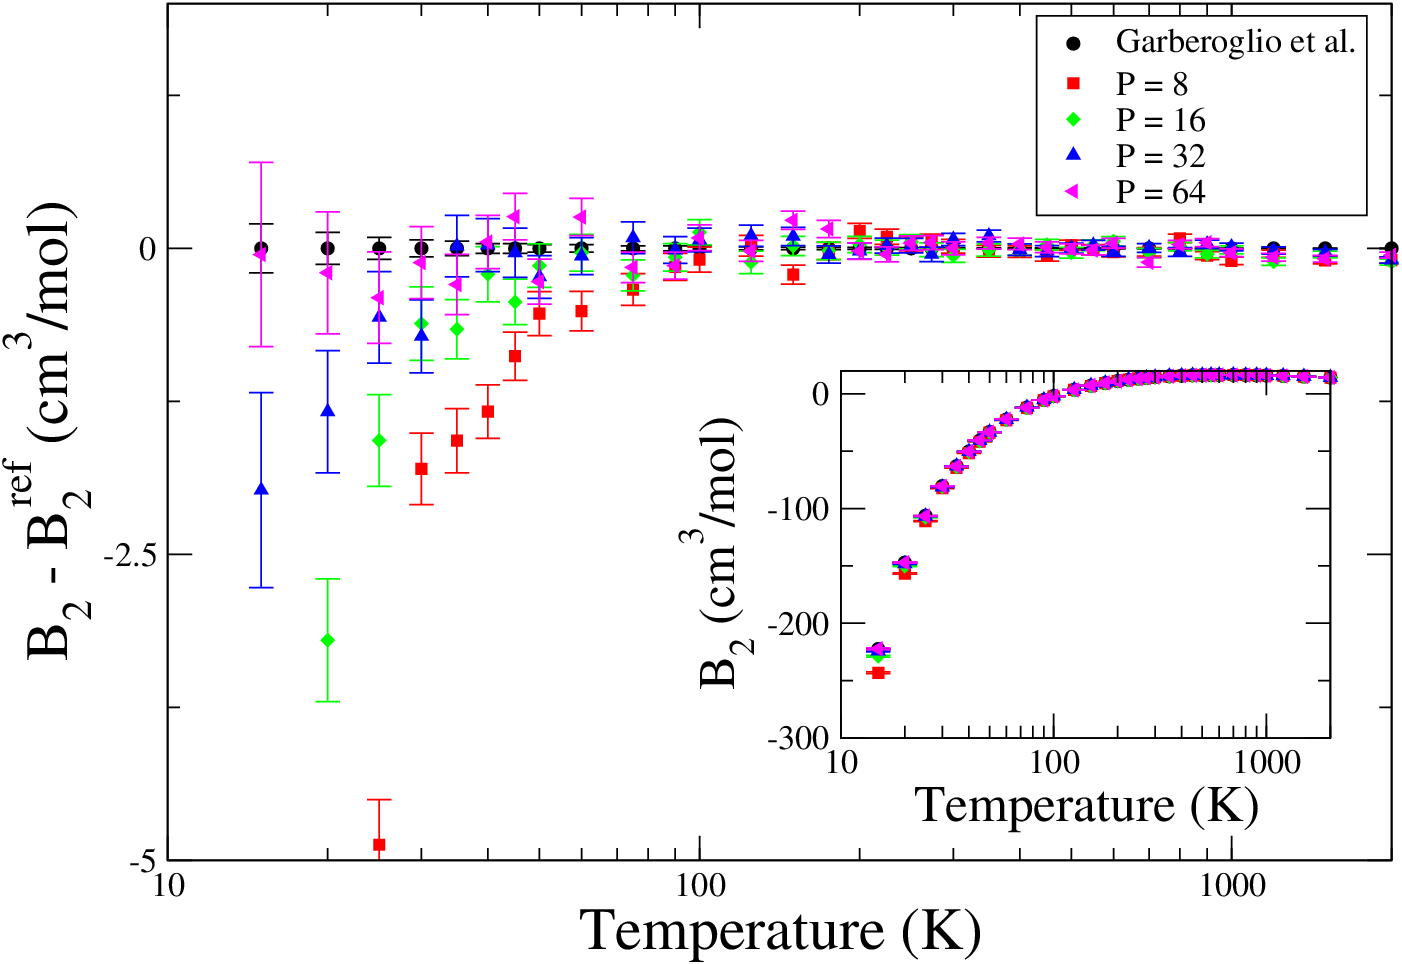
\includegraphics[width=10cm,keepaspectratio]{Chapter-4/Figures/s1GarberoglioAll.png}
                    \caption{Fully quantum second virial coefficient ($B_2$) values compared against reference values \cite{Garberoglio2014}, for Model 1. Main figure is the difference between the values computed here and the reference values, while the inset shows the coefficients before differencing. The value of the number of path-integral beads is $P$, and the results for different $P$ are as indicated in the legend. Error bars represent one standard deviation of the mean (68\% confidence interval). Low-temperature values for $P = 8$ and 16 are off the bottom of the scale.}
                    \label{fig:r0}
                \end{figure}
                In Fig. \ref{fig:r0} we show our $B_2$ values and the reference values for Model 1 as a function of temperature. It can be seen that the agreement between reference values and our results is generally good over the wide range of temperatures considered (15 K to 2000 K). The agreement is particularly good for $T > 50 $K where our results using $P = 64$ images are sufficient to achieve convergence according to Eq. \eqref{eq:s1P}. For $T \le 50 $K, we observe statistically significant disagreement between our results (for all $P$ considered) and reference values, and the magnitude of this deviation decreases with increasing $P$ and/or $T$. As explained earlier, this behavior is expected because the number of images we use is not sufficient for convergence according to Eq. \eqref{eq:s1P}.

                \begin{figure}[!htbp]
                    \centering
                    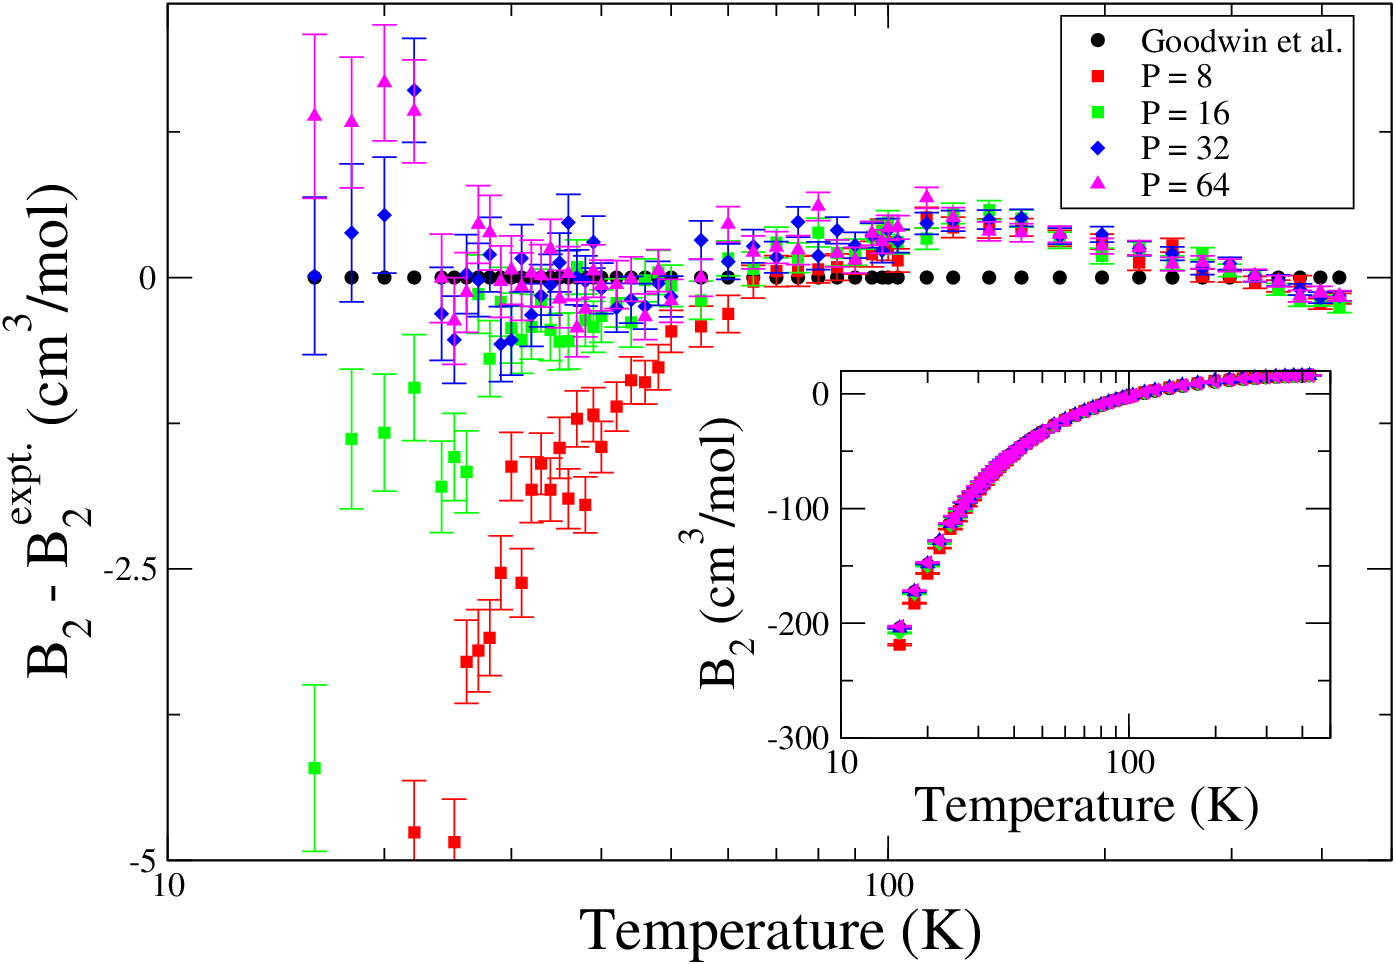
\includegraphics[scale=0.20,keepaspectratio]{Chapter-4/Figures/s1GoodwinAll.png}
                    \caption{Same as Fig. \ref{fig:r0}, but with comparison made to experimental data of Goodwin et al.\cite{Goodwin1963} rather than computed values from \cite{Garberoglio2014}. Low-temperature values for $P = 8$ and 16 are off the bottom of the scale.}
                    \label{fig:r0Goodwin}
                \end{figure}
                In Fig. \ref{fig:r0Goodwin} we compare our $B_2$ values for Model 1 against experimental results of Goodwin et al.\cite{Goodwin1963}. We observe particularly good agreement in two ranges of temperatures, $24 K \le T \le 50 $K and $ 248.15 K \le T \le 423.15 $K, and significant deviations for other temperatures. Since we expect our results to have not converged for $T \le 50 $K, we consider the agreement in the range $24 K \le T \le 50 $K to be fortuitous. At the higher temperature range where our results are converged according to Eq. \eqref{eq:s1P}, the agreement is of course expected. One possible reason for the disagreement observed at higher temperatures could be due to poor quality of the function fitted to experimental data at these temperatures. The disagreement observed at lower temperatures can be attributed to calculations involving insufficient $P$.

                \begin{figure}[!htbp]
                    \centering
                    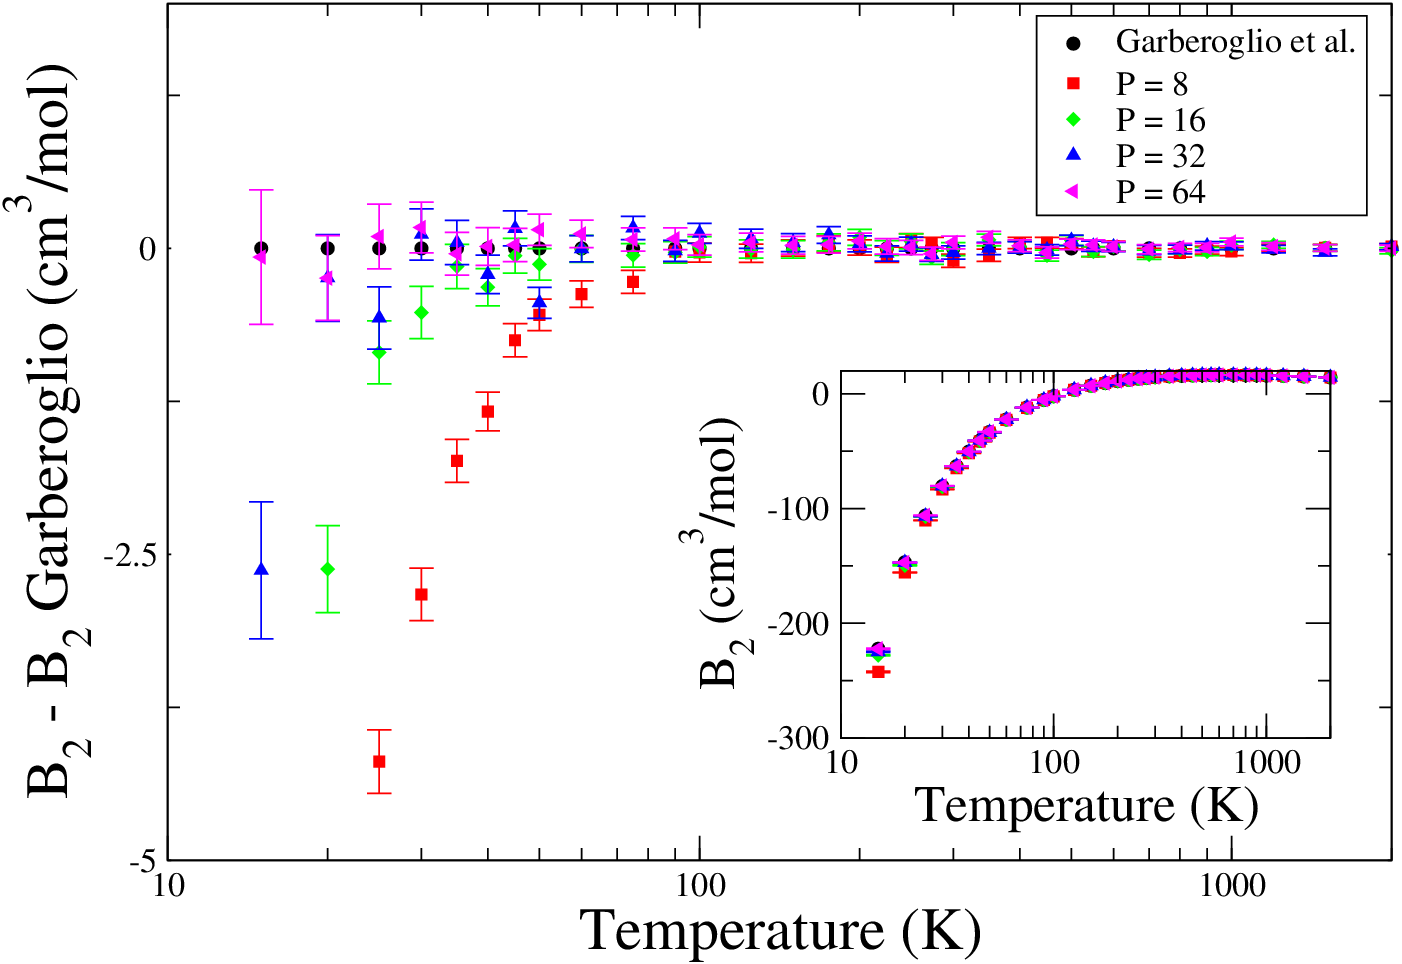
\includegraphics[scale=0.20,keepaspectratio]{Chapter-4/Figures/s2GarberoglioAll.png}
                    \caption{Same as Fig. \ref{fig:r0}, but values shown are those computed for Model 2 rather than Model 1. Error bars represent one standard deviation of the mean (68\% confidence interval). Low-temperature values for $P = 8$ and 16 are off the bottom of the scale.}
                    \label{fig:rT}
                \end{figure}
                In Fig. \ref{fig:rT} we show our $B_2$ values and the reference values for Model 2 as a function of temperature. It can be seen that the agreement between reference values and our results is particularly good for all temperatures except $T = 15$ K and $25$ K, where our results have not converged in $P$ (in accordance with Eq. \eqref{eq:s2P}). For a few temperatures below 40 K, we point out that our results have converged using fewer $P$ than that prescribed by Eq. \eqref{eq:s2P}.

            \subsubsection{Orientation algorithm performance}
                \label{sec:orPerformance}
                \begin{figure}[!htbp]
                    \centering
                    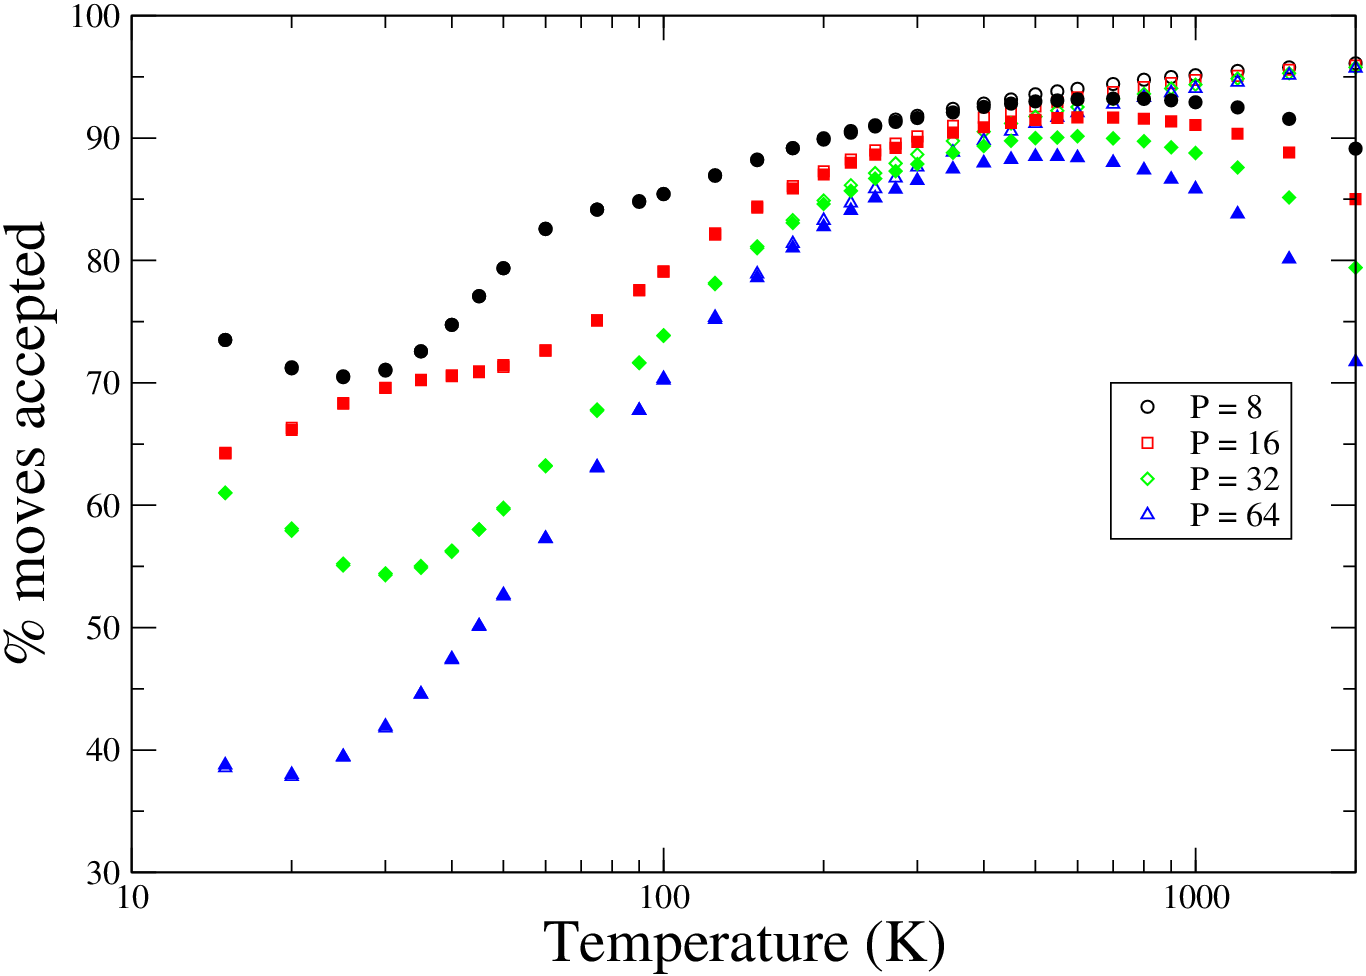
\includegraphics[scale=0.20,keepaspectratio]{Chapter-4/Figures/s12orAcc.png}
                    \caption{Performance of the orientation move for models 1 and 2. Values for model 1 are represented using open symbols while that for model 2 are represented using filled symbols with the same shape.}
                    \label{fig:r0Acc}
                \end{figure}

                In fig. \ref{fig:r0Acc} we show the percentage of orientation trials that were accepted, as a function of temperature for models 1 and 2. While we require more $P$ to accurately capture the nuclear quantum effects at low temperature, the efficiency of the algorithm decreases with increasing $P$. As explained earlier, this is because we achieve exact sampling of the angle $\alpha$ only for the $P/2$ images that are placed in the last step of the orientation algorithm. For the other $P/2$ images, the sampling is approximate and not exact. Still, the acceptance rate at all conditions is quite good, and in the worst case hovers around 40\%, which means that roughly two attempts at generating a configuration are required to produce one that is acceptable. Given that the new configuration is completely uncorrelated from the one preceding it, this represents a significant improvement in the efficiency of sampling of the path-integral conformations.

                Fig. \ref{fig:r0Acc} shows that there is a significant change in the behavior of the acceptance rate for models 1 and 2 for the higher temperatures, where the performance for the model 1 case is increasing while that of model 2 is decreasing with increasing $T$. To explain this behavior and gain further insight into the nature of the difference between the actual distribution $\pi({\mathbf b})$ (Eq. \eqref{eq:piTotal}) and the approximate distribution $\tau({\mathbf b}) (o \to n)$ (Eq. \eqref{eq:piTilde}), we performed a numerical study. We generated configurations of $P$ beads with probability $\pi({\bf{b}}^{\textrm{(B)}})$ using an exact but inefficient method (generating random positions on a sphere for all beads, and accepting with probability given by Eq.~\eqref{eq:piTotal}). We then tabulated the distribution of the angle $\alpha$ (as defined in Fig.~\ref{fig:simple}) for the first bead placed (thus, the case where beads A and B are the same, $\psi_{i,k} = 0$); the distribution of this angle is expected to differ most from that given by the approximation $\tau$. We performed this calculation for three values of $P$: 4, 8, 16, and three values of $k_h$: 0.5, 5.0, and 50.0 \AA$^{-2}$, which for H$_2$ correspond to temperatures (in K): $96.253/P, 962.53/P, 9625.3/P$, respectively. Comparisons to distributions of $\alpha$ for $\tau$ as given by Eq.~\eqref{eq:piTilde}  are plotted in Figs. \ref{fig:phi2B}, \ref{fig:phi4B} and \ref{fig:phi8B}.
                \begin{itemize}
                    \item For a given $P$, we observe that the approximate distribution seems to be under-predicting for some range of angles and over-predicting for other ranges, as it must for both distributions to be normalized.
                    \item For a given $P$, the actual distribution gets narrower and taller as we increase $k_h$. This is to be expected because springs with high $k_h$ values tend to prefer smaller angles $\alpha$ as they are harmonically more favorable. The generally increasing trend in the percentage moves accepted as a function of temperature (as seen in fig. \ref{fig:r0Acc}) can be explained due to this phenomenon as $k_h$ is directly proportional to $T$.
                \end{itemize}

                \begin{figure}[!htbp]
                    \centering
                    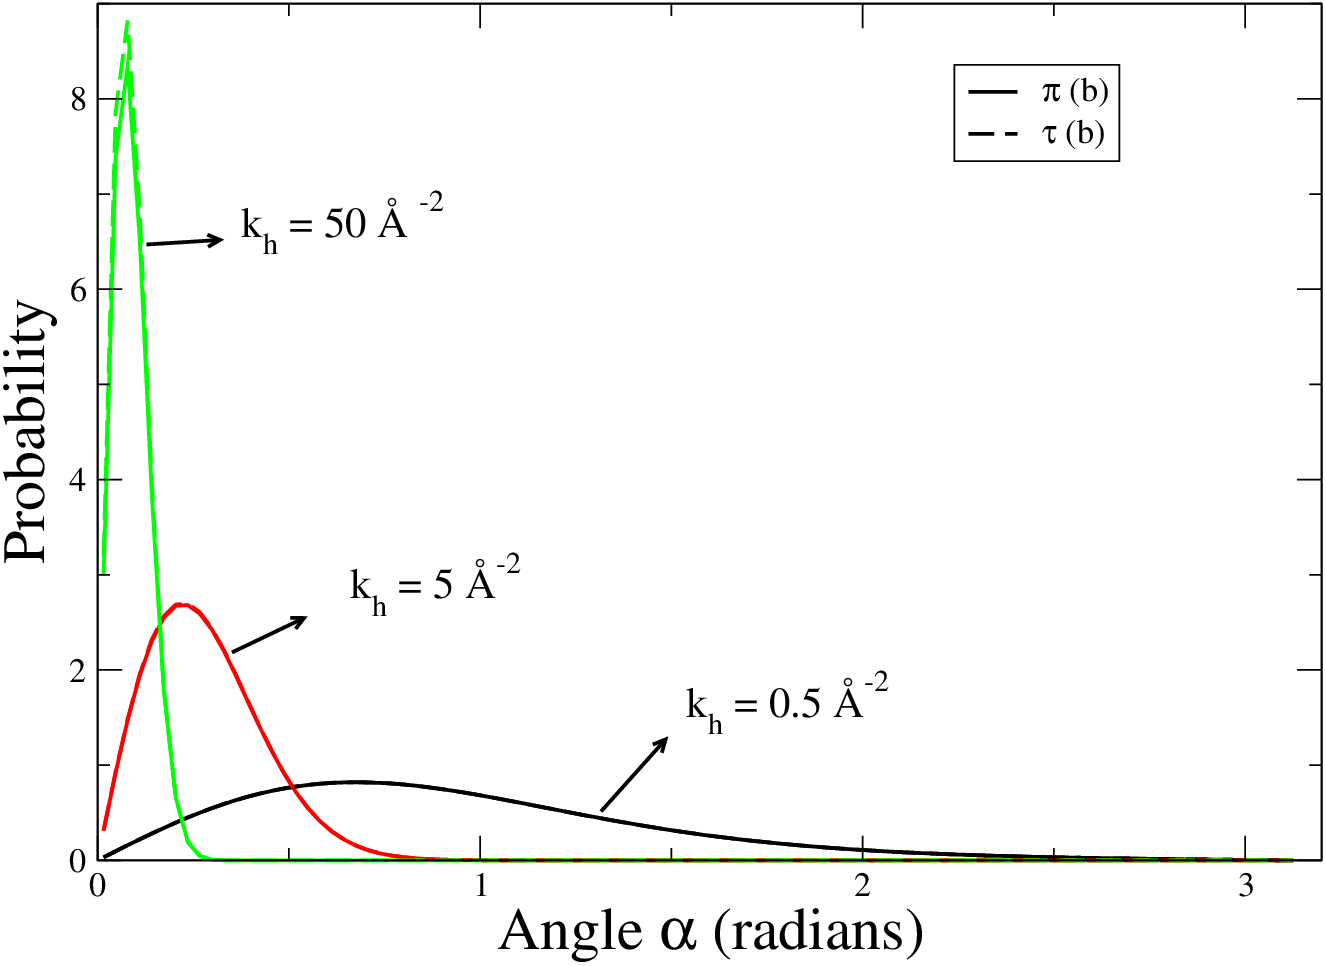
\includegraphics[scale=0.20,keepaspectratio]{Chapter-4/Figures/phi2B.png}
                    \caption{Approximate and actual probability distributions for $P =$ 4.}
                    \label{fig:phi2B}
                \end{figure}

                \begin{figure}[!htbp]
                    \centering
                    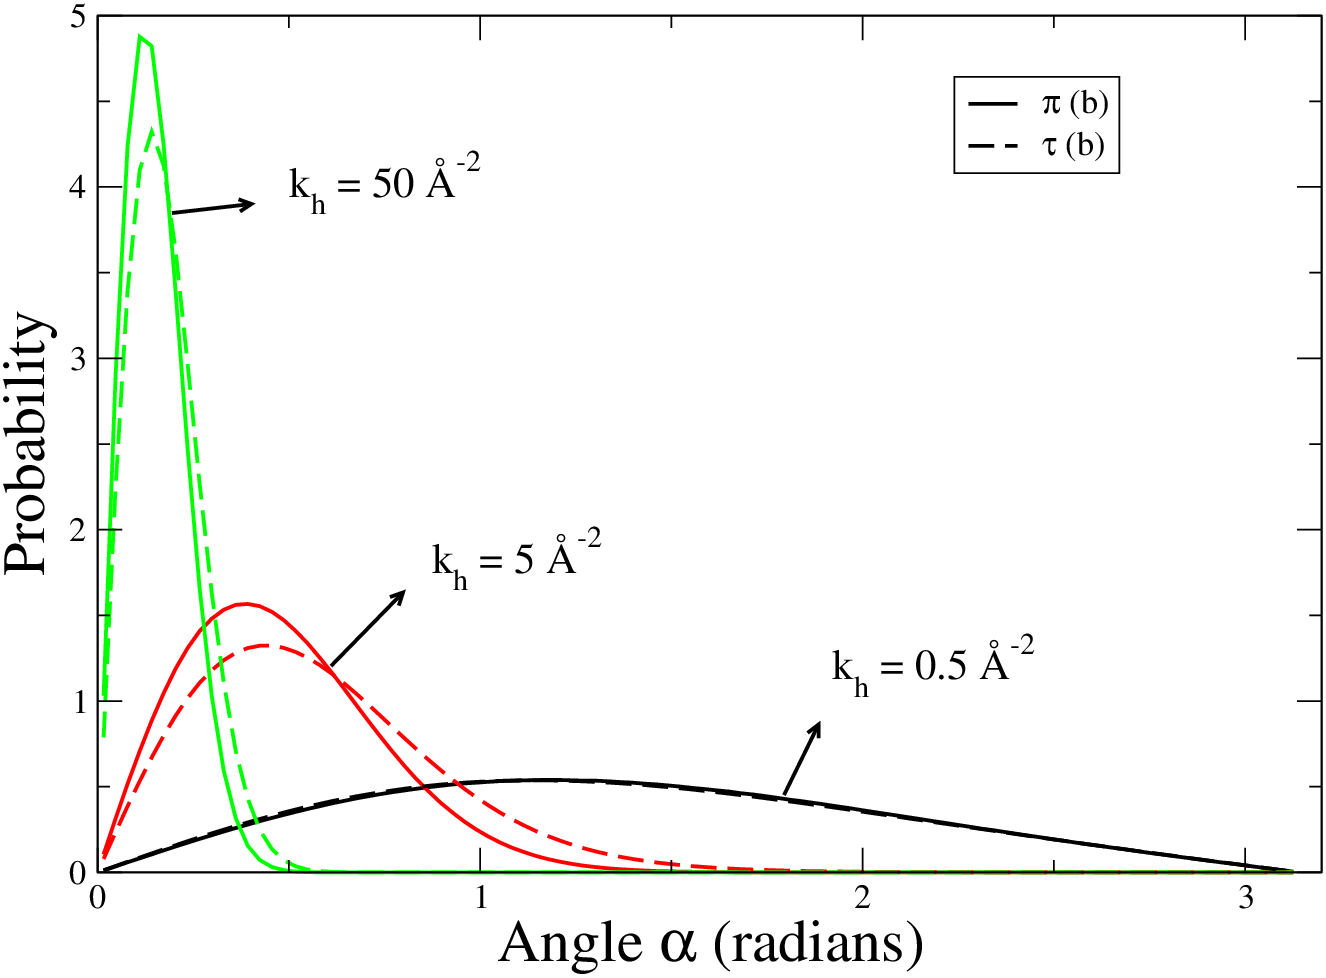
\includegraphics[scale=0.20,keepaspectratio]{Chapter-4/Figures/phi4B.png}
                    \caption{Approximate and actual probability distributions for $P =$ 8.}
                    \label{fig:phi4B}
                \end{figure}

                \begin{figure}[!htbp]
                    \centering
                    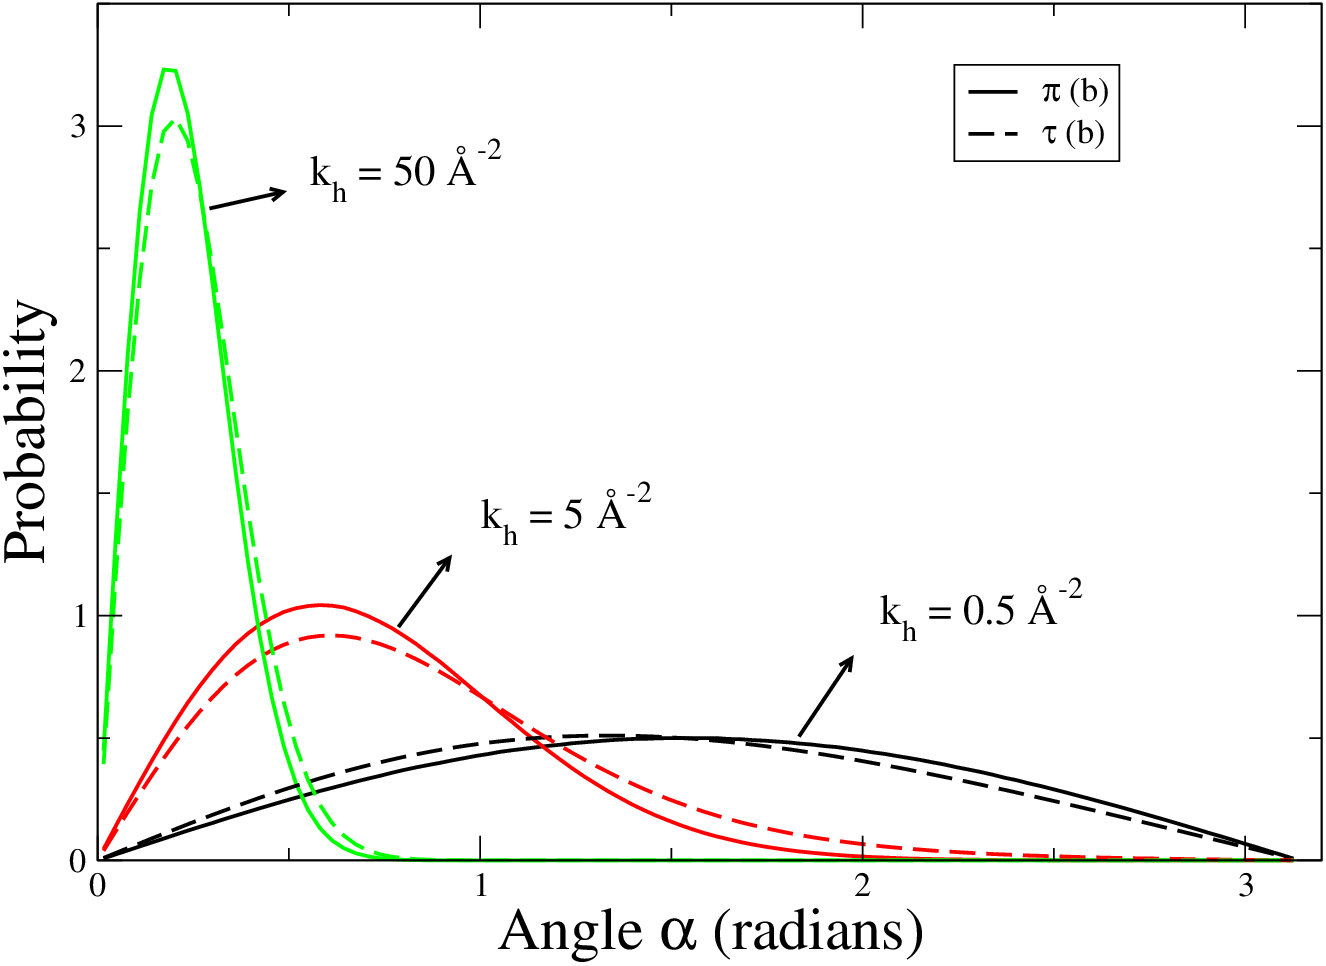
\includegraphics[scale=0.20,keepaspectratio]{Chapter-4/Figures/phi8B.png}
                    \caption{Approximate and actual probability distributions for $P =$ 16.}
                    \label{fig:phi8B}
                \end{figure}

                To further elucidate the difference between the approximate and actual distributions, we plot the ratio of the actual and the approximate distributions on the $y$-axis and the approximate distribution on the $x$-axis for the various $P$ and $k_h$ values examined above. This ratio is exactly the quantity entering into the acceptance probability of the configuration, as given by Eq~\eqref{eq:Pacc}. For ease of explanation, we define ``closeness" between the two distributions as the deviation of $y$-coordinate from the $y = 1$ line in figs. \ref{fig:ratio2B}, \ref{fig:ratio4B} and \ref{fig:ratio8B}. It is worth remembering that the distributions plotted here are for just the first bead placement, and that the overall acceptance of a trial configuration is given as the product of functions like these for all subsequent bead placements.

                \begin{figure}[!htbp]
                    \centering
                    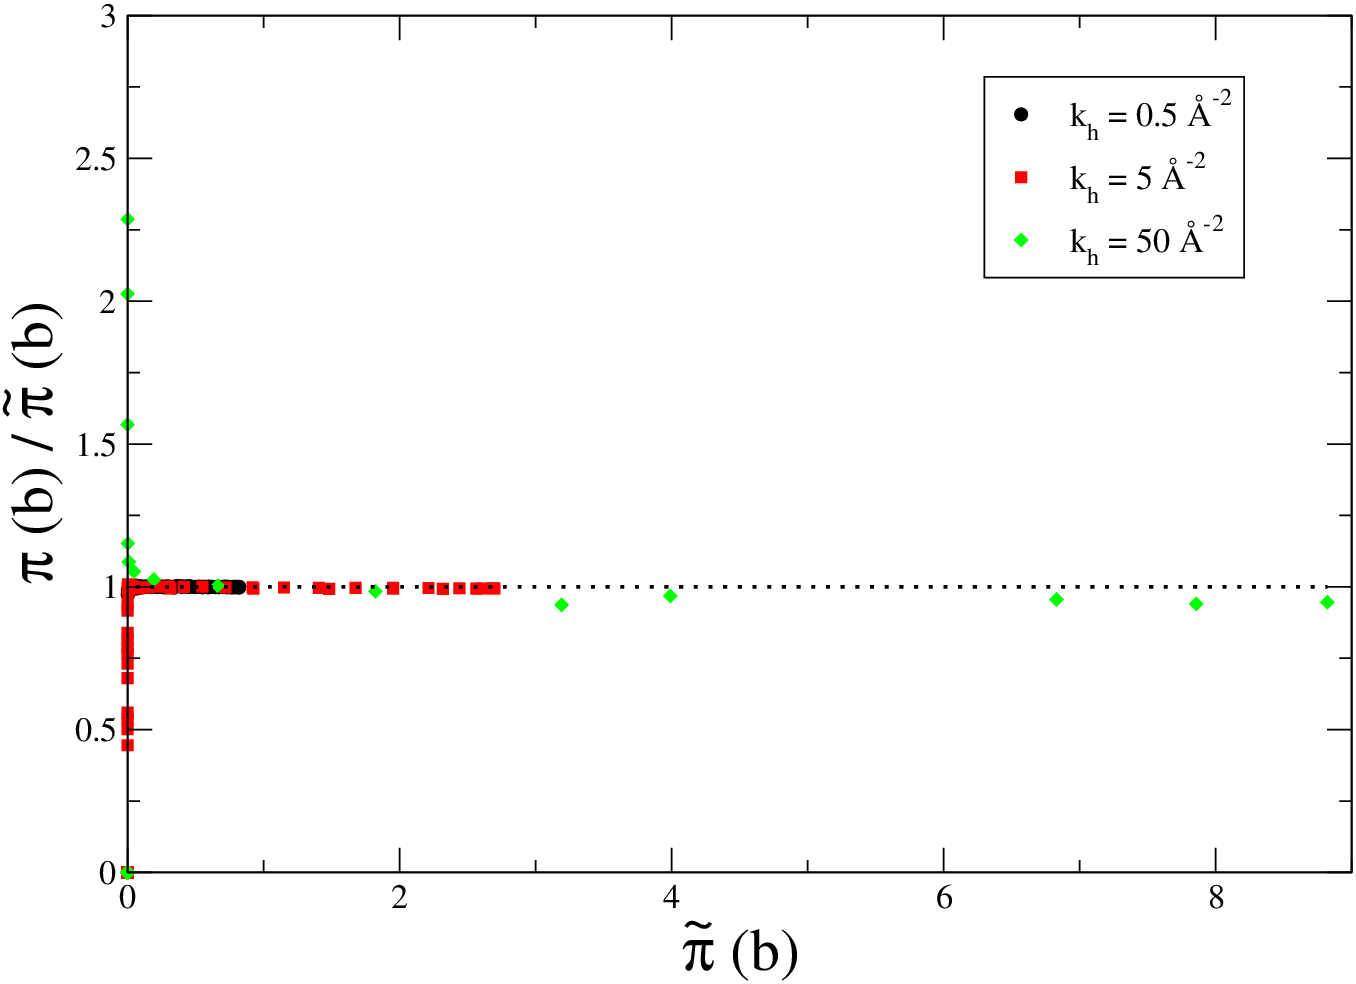
\includegraphics[scale=0.20,keepaspectratio]{Chapter-4/Figures/ratio2B.png}
                    \caption{Ratio of the approximate and actual probability distributions for $P =$ 4.}
                    \label{fig:ratio2B}
                \end{figure}

                \begin{figure}[!htbp]
                    \centering
                    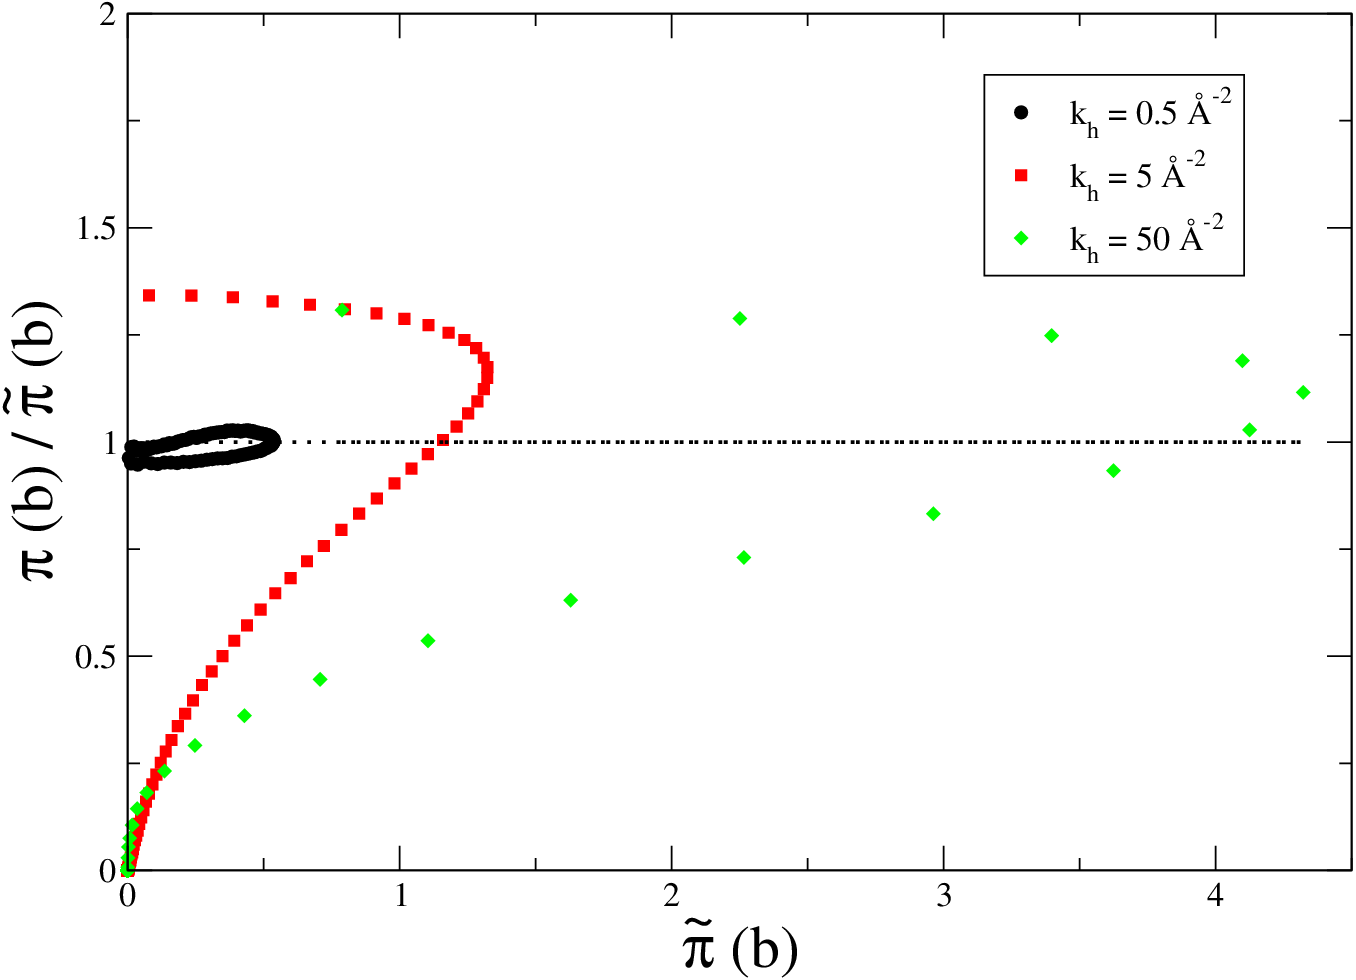
\includegraphics[scale=0.20,keepaspectratio]{Chapter-4/Figures/ratio4B.png}
                    \caption{Ratio of the approximate and actual probability distributions for $P =$ 8.}
                    \label{fig:ratio4B}
                \end{figure}

                \begin{figure}[!htbp]
                    \centering
                    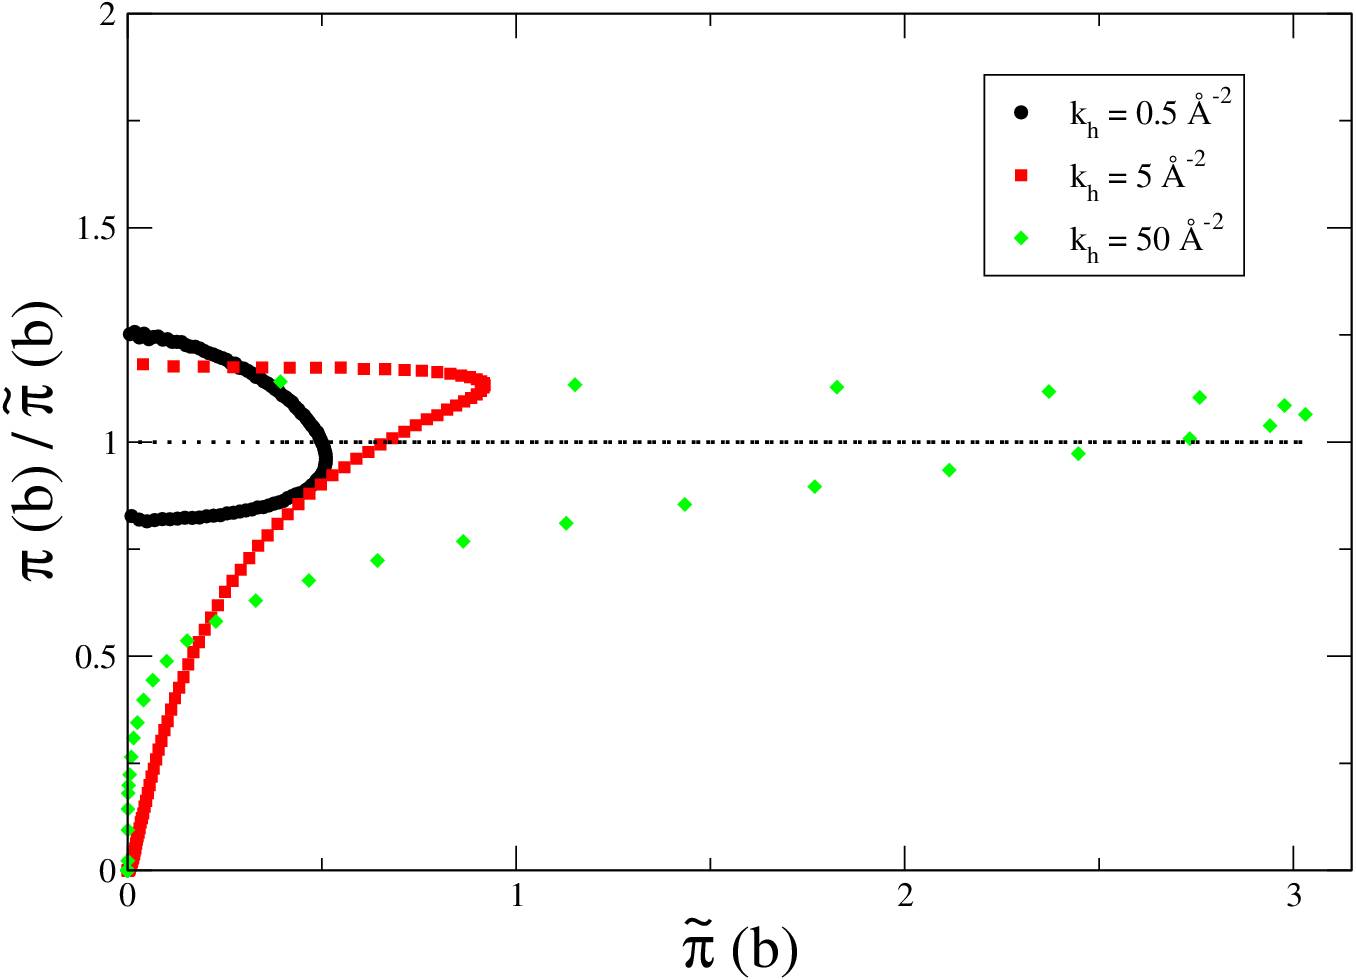
\includegraphics[scale=0.20,keepaspectratio]{Chapter-4/Figures/ratio8B.png}
                    \caption{Ratio of the approximate and actual probability distributions for $P =$ 16.}
                    \label{fig:ratio8B}
                \end{figure}

                From figs. \ref{fig:ratio2B}, \ref{fig:ratio4B} and \ref{fig:ratio8B}, we can infer the following:
                \begin{itemize}
                \item Severe problems would arise if the ratio $\pi/\tau$ were diverging for $\tau$ approaching zero, as this would indicate that there are configurations relevant to $\pi$ that are not sampled by the algorithm. The figures show that this problem does not arise.
                    \item In a related fashion, the points above the $y =1$ line indicate  that the actual distribution has been under-predicted by the approximate distribution and these points could potentially lead to configurations where the molecule is `stuck'. In other words, the probability of going from one of these points to a point on the $y =$ 1-line (favored) is very poor. However, this would happen only for $y \gg 1$, which is not observed in any of the cases.
                    \item In some cases, ``closeness" of the intermediate $k_h$ (= 5 \AA$^{-2}$) is worse than the other two cases, and this could lead to the minimum in fig. \ref{fig:r0Acc} because $k_h$ is directly proportional to temperature.
                \end{itemize}

        \subsection{Flexible-bond models -- Orientation and bond length trials}
            In this section we present and analyze the results for Model 3 (flexible-bond model) including the performance of the orientation-sampling trial and the bond length sampling trial when present simultaneously in a simulation. We begin by noting that the number of images used by Garberoglio for achieving converged results \cite{Garberoglio2014} for Model 3 was calculated as:
            \begin{equation}
            \label{eq:s3P}
                P = \lceil 7000 K/T + 8 \rceil
            \end{equation}
            where $\lceil x \rceil$ denotes the smallest integer larger than $x$.
According to Eq. \eqref{eq:s3P} the temperature at which we require $P > 64$ to achieve converged results for Model 3 is 100 K. Therefore we expect to see significant differences between our virial coefficient values for Model 3 and the corresponding reference values for $T \le 100 $K. Although for a given temperature $T$, Eq. \eqref{eq:s3P} provides a good estimate of $P$ required for achieving converged results, in practice, one might be able to achieve convergence with fewer $P$ as well.

            \subsubsection{$B_2$ values}
                \begin{figure}[!htbp]
                    \centering
                    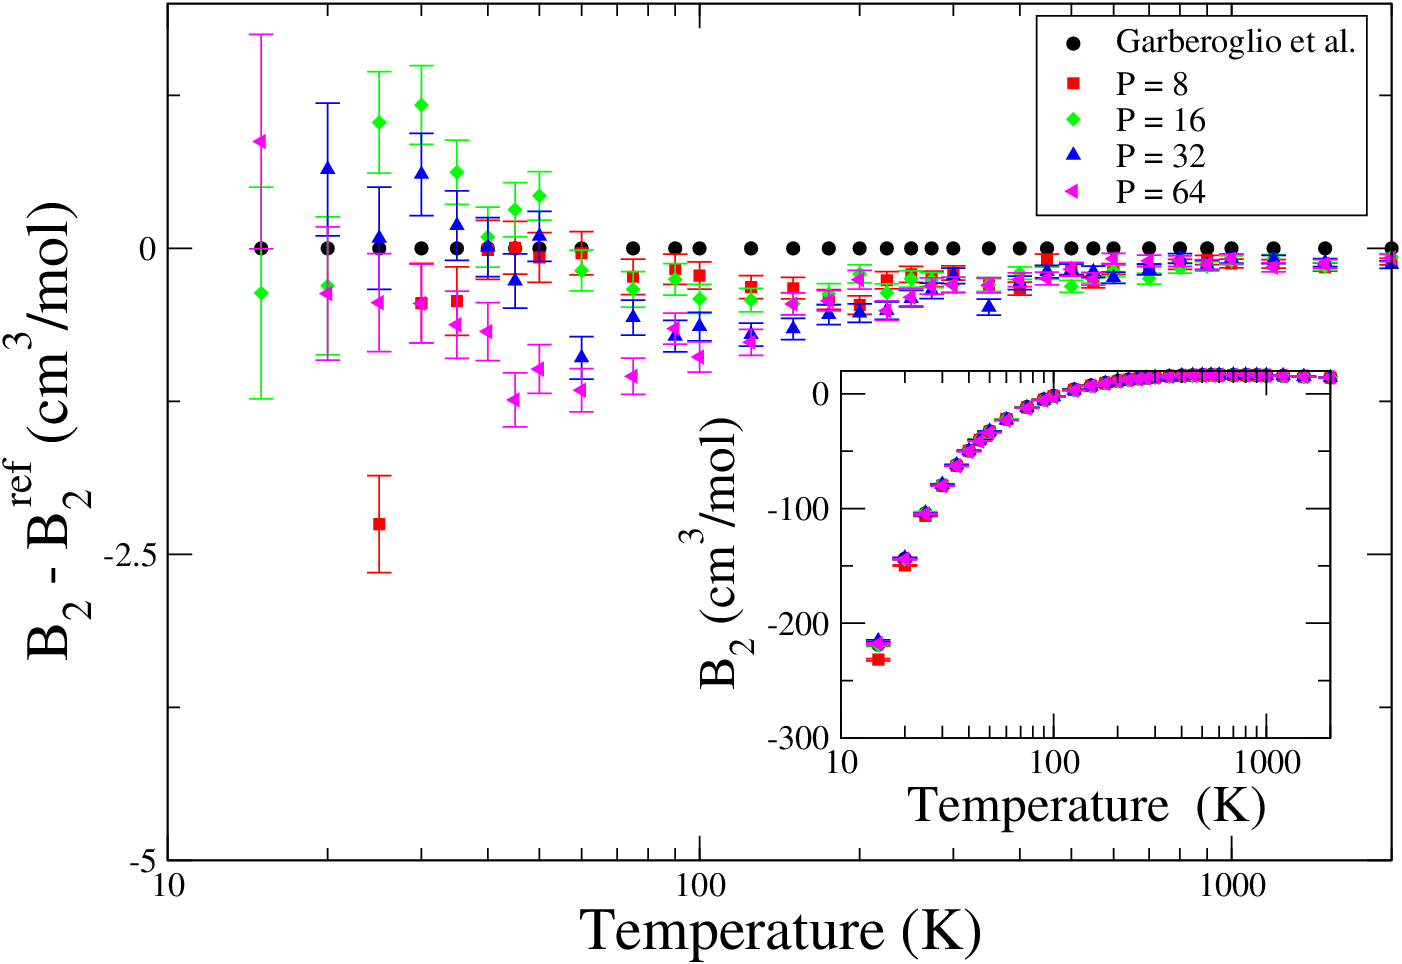
\includegraphics[scale=0.20,keepaspectratio]{Chapter-4/Figures/s3GarberoglioAll.png}
                    \caption{Fully quantum second virial coefficient ($B_2$) values compared against reference values \cite{Garberoglio2014}, for Model 3. Main figure is the difference between the values computed here and the reference values, while the inset shows the coefficients before differencing. The value of the number of path-integral beads is $P$, and the results for different $P$ are as indicated in the legend. Error bars represent one standard deviation of the mean (68\% confidence interval). Low-temperature values for $P = 8$ and 16 are off the bottom of the scale.}
                    \label{fig:variable}
                \end{figure}

                In Fig. \ref{fig:variable} we show our $B_2$ values and the reference values for Model 3 as a function of temperature. It can be seen that the agreement between reference values and our results is generally good over the wide range of temperatures considered (15 K to 2000 K). The agreement is particularly good for $T > 100 $K where our results using $P = 64$ images are sufficient enough to achieve convergence according to Eq. \eqref{eq:s3P}. For $T \le 100 $K, we observe statistically significant disagreement between our results (for all $P$ considered) and reference values and the magnitude of this deviation decreases with increasing $P$ and/or $T$ and vice-versa. As explained earlier, this behavior is expected because the number of images we use is not sufficient for convergence according to Eq. \eqref{eq:s3P}. The $P = 128$ and $256$ results show that upon systematically increasing the number of images, our values seem to approach the reference values.

            \subsubsection{Orientation algorithm performance}
                \begin{figure}[!htbp]
                    \centering
                    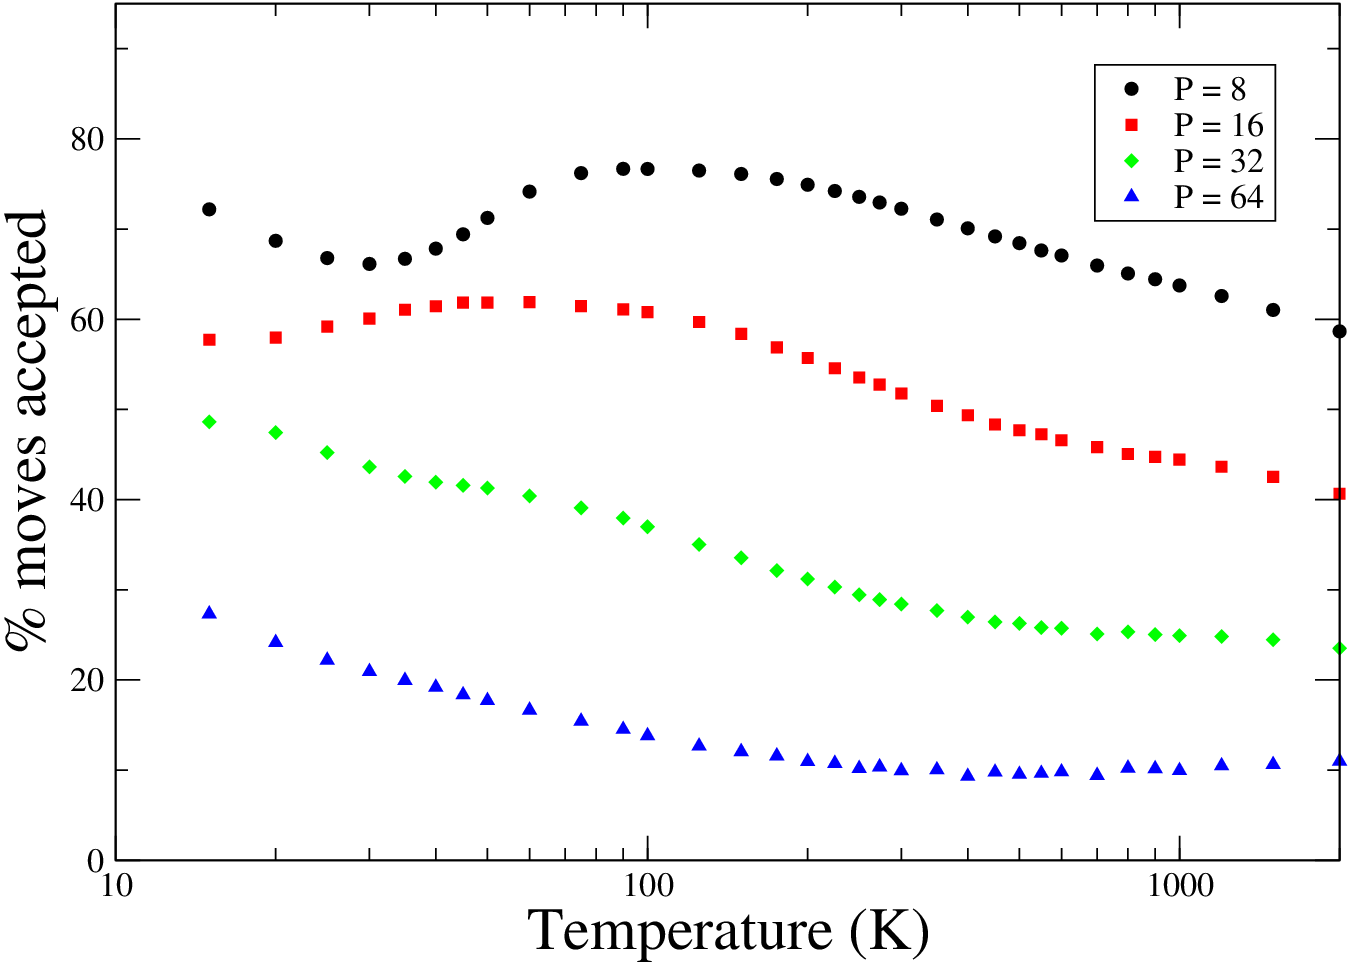
\includegraphics[scale=0.20,keepaspectratio]{Chapter-4/Figures/s3OrAcc.png}
                    \caption{Performance of the orientation move for model 3.}
                    \label{fig:variableOrAcc}
                \end{figure}

                In fig. \ref{fig:variableOrAcc} we have shown the percentage of orientation moves that were accepted as a function of temperature for model 3. We notice once again that the algorithm performance decreases with increasing $P$ which is to be expected because of the non-exact nature of the description of the $\alpha$ for $P/2$ images. In addition, we also observe that the performance of the orientation move is almost always worse in the presence of the bond length change move as can be seen in comparing figs. \ref{fig:r0Acc} and \ref{fig:variableOrAcc}. This can be attributed to the way we handle the bond lengths of different images being different within the orientation move. In its current implementation, we average the bond lengths of images $i$ through $k$ and use this value to place image $j$. However, this leads to using the incorrect value of the spring constant when computing the approximate distribution function, which in turn could lead to diminished percentage acceptance of the move.

            \subsubsection{Bond length algorithm performance}
                \label{sec:blPerformance}
                Before looking at the performance of the bond length algorithm, we present the following in support of our estimate of a representative angle $\hat \theta$ as given by Eq.~\eqref{eq:thetaHat}. We collected histograms of the average adjacent angle $\theta_{ij}$ during the course of model 1 simulations for $T = 15, 50, 100, 250$~and $500$ K and for $P = 8, 16, 32$~and $64$, and present the results in fig. \ref{fig:nominal_angle}. We can clearly see that Eq. \eqref{eq:thetaHat} over-predicts $\left<\theta_{ij}\right>$ slightly (about 10\%) for all cases, but given the simplicity and usefulness of the approximation, we can be satisfied with how well it tracks the dependence of the average angle with $T$ and $P$. We note that the difference seen in the figure affects only efficiency, not the accuracy of the calculations.
                \begin{figure}[!htbp]
                    \centering
                    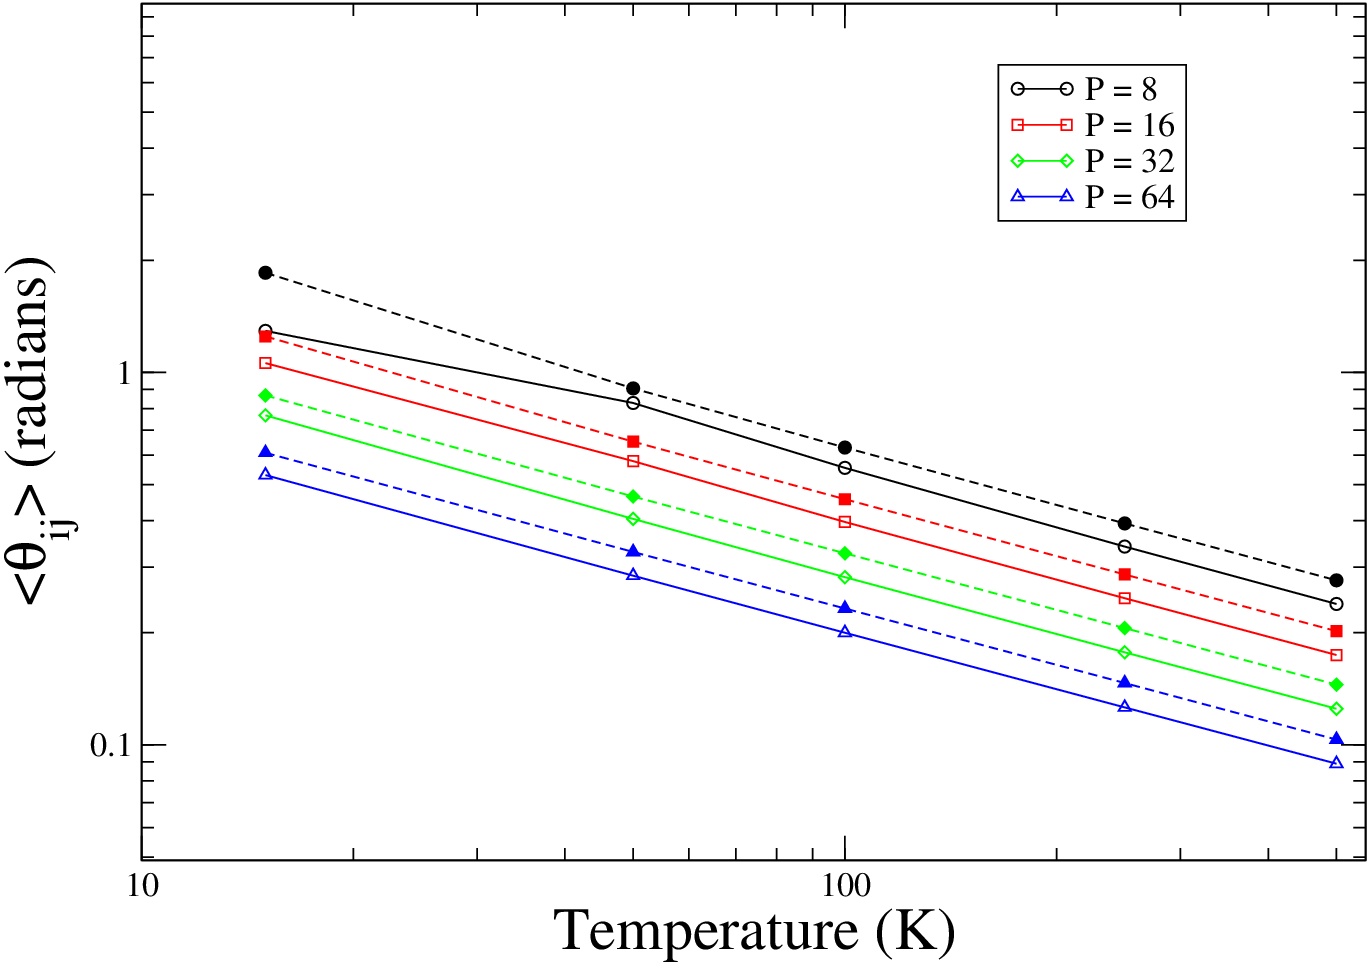
\includegraphics[scale=0.20,keepaspectratio]{Chapter-4/Figures/nominalAnglelogXlogY.png}
                    \caption{Nominal angle computed using eq. \eqref{eq:thetaHat} compared against average $\theta_{ij}$ observed in simulation. Open symbols connected by solid lines represent the $\left<\theta_{ij}\right>$ observed in simulation and filled symbols with the same shape connected by dashed lines represent the $\hat \theta$ computed using the formula given in eq. \eqref{eq:thetaHat}}
                    \label{fig:nominal_angle}
                \end{figure}

    \section{Conclusions}
        \label{sec:Conclusions and future work}
        We have demonstrated the algorithms developed in Secs. \ref{subsec:orMove} and \ref{subsec:blMove} by computing and comparing second virial coefficients for H$_2$ as a test case. We observed good agreement of our results with those available in literature for the three different cases explained in sec. \ref{sec:Computational details}. For lower temperatures ($T \le 100 $K), we concluded that a greater number of images $P$ were required to achieve results in better agreement with literature. We emphasize that the failure to converge using insufficient $P$ is an artifact of quantum mechanics and not the orientation sampling algorithm. Although such an analysis was not attempted for the case of the bond length trial for the test case of H$_2$, we suspect that these might become necessary in the future for other molecules, where the performance of the bond length sampling algorithm might not be considered satisfactory. Based on our observation, the orientation move always performs better than the bond length move and the presence of the bond length move always decreases the performance of the orientation move.

    \section{Tabulated Results}
    \label{sec:chap4-tables}
        We report tabulated results for primarily the virial coefficients of hydrogen and other related quantities in this section.
        \pgfplotstableset{
            begin table=\begin{longtable},
            end table=\end{longtable},
        }
        \pgfkeys{
        /pgf/number format/.cd,
        sci,
        sci generic={mantissa sep=\times,exponent={10^{#1}}}
        }
        \pgfplotstabletypeset[
            columns/temperature/.style={
                string type,
                column name={Temperature(\si{\kelvin})}
            },
            columns/ratio/.style={
                string type,
                column name=Ratio($Q_1^\text{xc}/Q_1^\text{B}$)
            },
            every head row/.append style={before row={\caption{Ratio of the partition function for exchange and Boltzmann type conformations used in virial coefficient calculations. These ratios were obtained using the values in Fig. 2 of Ref \cite{Garberoglio2014} that were fitted to different temperatures.}\label{tab:xcBRatios}\\\toprule},after row=\midrule\endfirsthead},
            every first row/.append style={before row={\multicolumn{2}{c}{\tablename\ \thetable{} -- Continued from previous page.}\\\toprule},after row=\midrule\endhead},
            every last row/.style={after row=\bottomrule},
        ]{Chapter-4/Tables/xcBRatios.e}

        \pgfplotstabletypeset[
            columns/temperature/.style={
                string type,
                column name={Temperature(\si{\kelvin})}
            },
            columns/b2xc/.style={
                string type,
                column name=B$^\text{xc}_2$(\si{cm^3/mol})
            },
            columns/b2b/.style={
                string type,
                column name=B$^\text{B}_2$(\si{cm^3/mol})
            },
            columns/b2tot/.style={
                string type,
                column name=B$^\text{Tot}_2$(\si{cm^3/mol})
            },
            every head row/.append style={before row={\caption{Second virial coefficient of hydrogen as a function of temperature for $P$ = 8 and Model 1. B$_2^\text{xc}$ and B$^\text{B}_2$ represent the exchange and Boltzmann contributions respectively, to the second virial coefficient. B$^\text{Tot}_2$ represents the final value for any temperature computed by combining the exchange and Boltzmann contributions according to the corresponding ratio from Table \ref{tab:xcBRatios}. Values in parantheses are standard uncertainties in the rightmost digit(s).}\label{tab:8nbs1Results}\\\toprule},after row=\midrule\endfirsthead},
            every first row/.append style={before row={\multicolumn{2}{c}{\tablename\ \thetable{} -- Continued from previous page.}\\\toprule},after row=\midrule\endhead},
            every last row/.style={after row=\bottomrule},
        ]{Chapter-4/Tables/8nbs1ResultsTable.dat}

        \pgfplotstabletypeset[
            columns/temperature/.style={
                string type,
                column name={Temperature(\si{\kelvin})}
            },
            columns/b2xc/.style={
                string type,
                column name=B$^\text{xc}_2$(\si{cm^3/mol})
            },
            columns/b2b/.style={
                string type,
                column name=B$^\text{B}_2$(\si{cm^3/mol})
            },
            columns/b2tot/.style={
                string type,
                column name=B$^\text{Tot}_2$(\si{cm^3/mol})
            },
            every head row/.append style={before row={\caption{Second virial coefficient of hydrogen as a function of temperature for $P$ = 16 and Model 1. B$_2^\text{xc}$ and B$^\text{B}_2$ represent the exchange and Boltzmann contributions respectively, to the second virial coefficient. B$^\text{Tot}_2$ represents the final value for any temperature computed by combining the exchange and Boltzmann contributions according to the corresponding ratio from Table \ref{tab:xcBRatios}. Values in parantheses are standard uncertainties in the rightmost digit(s).}\label{tab:16nbs1Results}\\\toprule},after row=\midrule\endfirsthead},
            every first row/.append style={before row={\multicolumn{2}{c}{\tablename\ \thetable{} -- Continued from previous page.}\\\toprule},after row=\midrule\endhead},
            every last row/.style={after row=\bottomrule},
        ]{Chapter-4/Tables/16nbs1ResultsTable.dat}

        \pgfplotstabletypeset[
            columns/temperature/.style={
                string type,
                column name={Temperature(\si{\kelvin})}
            },
            columns/b2xc/.style={
                string type,
                column name=B$^\text{xc}_2$(\si{cm^3/mol})
            },
            columns/b2b/.style={
                string type,
                column name=B$^\text{B}_2$(\si{cm^3/mol})
            },
            columns/b2tot/.style={
                string type,
                column name=B$^\text{Tot}_2$(\si{cm^3/mol})
            },
            every head row/.append style={before row={\caption{Second virial coefficient of hydrogen as a function of temperature for $P$ = 32 and Model 1. B$_2^\text{xc}$ and B$^\text{B}_2$ represent the exchange and Boltzmann contributions respectively, to the second virial coefficient. B$^\text{Tot}_2$ represents the final value for any temperature computed by combining the exchange and Boltzmann contributions according to the corresponding ratio from Table \ref{tab:xcBRatios}. Values in parantheses are standard uncertainties in the rightmost digit(s).}\label{tab:32nbs1Results}\\\toprule},after row=\midrule\endfirsthead},
            every first row/.append style={before row={\multicolumn{2}{c}{\tablename\ \thetable{} -- Continued from previous page.}\\\toprule},after row=\midrule\endhead},
            every last row/.style={after row=\bottomrule},
        ]{Chapter-4/Tables/32nbs1ResultsTable.dat}

        \pgfplotstabletypeset[
            columns/temperature/.style={
                string type,
                column name={Temperature(\si{\kelvin})}
            },
            columns/b2xc/.style={
                string type,
                column name=B$^\text{xc}_2$(\si{cm^3/mol})
            },
            columns/b2b/.style={
                string type,
                column name=B$^\text{B}_2$(\si{cm^3/mol})
            },
            columns/b2tot/.style={
                string type,
                column name=B$^\text{Tot}_2$(\si{cm^3/mol})
            },
            every head row/.append style={before row={\caption{Second virial coefficient of hydrogen as a function of temperature for $P$ = 64 and Model 1. B$_2^\text{xc}$ and B$^\text{B}_2$ represent the exchange and Boltzmann contributions respectively, to the second virial coefficient. B$^\text{Tot}_2$ represents the final value for any temperature computed by combining the exchange and Boltzmann contributions according to the corresponding ratio from Table \ref{tab:xcBRatios}. Values in parantheses are standard uncertainties in the rightmost digit(s).}\label{tab:64nbs1Results}\\\toprule},after row=\midrule\endfirsthead},
            every first row/.append style={before row={\multicolumn{2}{c}{\tablename\ \thetable{} -- Continued from previous page.}\\\toprule},after row=\midrule\endhead},
            every last row/.style={after row=\bottomrule},
        ]{Chapter-4/Tables/64nbs1ResultsTable.dat}

        \pgfplotstabletypeset[
            columns/temperature/.style={
                string type,
                column name={Temperature(\si{\kelvin})}
            },
            columns/b2xc/.style={
                string type,
                column name=B$^\text{xc}_2$(\si{cm^3/mol})
            },
            columns/b2b/.style={
                string type,
                column name=B$^\text{B}_2$(\si{cm^3/mol})
            },
            columns/b2tot/.style={
                string type,
                column name=B$^\text{Tot}_2$(\si{cm^3/mol})
            },
            every head row/.append style={before row={\caption{Second virial coefficient of hydrogen as a function of temperature for $P$ = 8 and Model 2. B$_2^\text{xc}$ and B$^\text{B}_2$ represent the exchange and Boltzmann contributions respectively, to the second virial coefficient. B$^\text{Tot}_2$ represents the final value for any temperature computed by combining the exchange and Boltzmann contributions according to the corresponding ratio from Table \ref{tab:xcBRatios}. Values in parantheses are standard uncertainties in the rightmost digit(s).}\label{tab:8nbs2Results}\\\toprule},after row=\midrule\endfirsthead},
            every first row/.append style={before row={\multicolumn{2}{c}{\tablename\ \thetable{} -- Continued from previous page.}\\\toprule},after row=\midrule\endhead},
            every last row/.style={after row=\bottomrule},
        ]{Chapter-4/Tables/8nbs2ResultsTable.dat}

        \pgfplotstabletypeset[
            columns/temperature/.style={
                string type,
                column name={Temperature(\si{\kelvin})}
            },
            columns/b2xc/.style={
                string type,
                column name=B$^\text{xc}_2$(\si{cm^3/mol})
            },
            columns/b2b/.style={
                string type,
                column name=B$^\text{B}_2$(\si{cm^3/mol})
            },
            columns/b2tot/.style={
                string type,
                column name=B$^\text{Tot}_2$(\si{cm^3/mol})
            },
            every head row/.append style={before row={\caption{Second virial coefficient of hydrogen as a function of temperature for $P$ = 16 and Model 2. B$_2^\text{xc}$ and B$^\text{B}_2$ represent the exchange and Boltzmann contributions respectively, to the second virial coefficient. B$^\text{Tot}_2$ represents the final value for any temperature computed by combining the exchange and Boltzmann contributions according to the corresponding ratio from Table \ref{tab:xcBRatios}. Values in parantheses are standard uncertainties in the rightmost digit(s).}\label{tab:16nbs2Results}\\\toprule},after row=\midrule\endfirsthead},
            every first row/.append style={before row={\multicolumn{2}{c}{\tablename\ \thetable{} -- Continued from previous page.}\\\toprule},after row=\midrule\endhead},
            every last row/.style={after row=\bottomrule},
        ]{Chapter-4/Tables/16nbs2ResultsTable.dat}

        \pgfplotstabletypeset[
            columns/temperature/.style={
                string type,
                column name={Temperature(\si{\kelvin})}
            },
            columns/b2xc/.style={
                string type,
                column name=B$^\text{xc}_2$(\si{cm^3/mol})
            },
            columns/b2b/.style={
                string type,
                column name=B$^\text{B}_2$(\si{cm^3/mol})
            },
            columns/b2tot/.style={
                string type,
                column name=B$^\text{Tot}_2$(\si{cm^3/mol})
            },
            every head row/.append style={before row={\caption{Second virial coefficient of hydrogen as a function of temperature for $P$ = 32 and Model 2. B$_2^\text{xc}$ and B$^\text{B}_2$ represent the exchange and Boltzmann contributions respectively, to the second virial coefficient. B$^\text{Tot}_2$ represents the final value for any temperature computed by combining the exchange and Boltzmann contributions according to the corresponding ratio from Table \ref{tab:xcBRatios}. Values in parantheses are standard uncertainties in the rightmost digit(s).}\label{tab:32nbs2Results}\\\toprule},after row=\midrule\endfirsthead},
            every first row/.append style={before row={\multicolumn{2}{c}{\tablename\ \thetable{} -- Continued from previous page.}\\\toprule},after row=\midrule\endhead},
            every last row/.style={after row=\bottomrule},
        ]{Chapter-4/Tables/32nbs2ResultsTable.dat}

        \pgfplotstabletypeset[
            columns/temperature/.style={
                string type,
                column name={Temperature(\si{\kelvin})}
            },
            columns/b2xc/.style={
                string type,
                column name=B$^\text{xc}_2$(\si{cm^3/mol})
            },
            columns/b2b/.style={
                string type,
                column name=B$^\text{B}_2$(\si{cm^3/mol})
            },
            columns/b2tot/.style={
                string type,
                column name=B$^\text{Tot}_2$(\si{cm^3/mol})
            },
            every head row/.append style={before row={\caption{Second virial coefficient of hydrogen as a function of temperature for $P$ = 64 and Model 2. B$_2^\text{xc}$ and B$^\text{B}_2$ represent the exchange and Boltzmann contributions respectively, to the second virial coefficient. B$^\text{Tot}_2$ represents the final value for any temperature computed by combining the exchange and Boltzmann contributions according to the corresponding ratio from Table \ref{tab:xcBRatios}. Values in parantheses are standard uncertainties in the rightmost digit(s).}\label{tab:64nbs2Results}\\\toprule},after row=\midrule\endfirsthead},
            every first row/.append style={before row={\multicolumn{2}{c}{\tablename\ \thetable{} -- Continued from previous page.}\\\toprule},after row=\midrule\endhead},
            every last row/.style={after row=\bottomrule},
        ]{Chapter-4/Tables/64nbs2ResultsTable.dat}

        \pgfplotstabletypeset[
            columns/temperature/.style={
                string type,
                column name={Temperature(\si{\kelvin})}
            },
            columns/b2xc/.style={
                string type,
                column name=B$^\text{xc}_2$(\si{cm^3/mol})
            },
            columns/b2b/.style={
                string type,
                column name=B$^\text{B}_2$(\si{cm^3/mol})
            },
            columns/b2tot/.style={
                string type,
                column name=B$^\text{Tot}_2$(\si{cm^3/mol})
            },
            every head row/.append style={before row={\caption{Second virial coefficient of hydrogen as a function of temperature for $P$ = 8 and Model 3. B$_2^\text{xc}$ and B$^\text{B}_2$ represent the exchange and Boltzmann contributions respectively, to the second virial coefficient. B$^\text{Tot}_2$ represents the final value for any temperature computed by combining the exchange and Boltzmann contributions according to the corresponding ratio from Table \ref{tab:xcBRatios}. Values in parantheses are standard uncertainties in the rightmost digit(s).}\label{tab:8nbs3Results}\\\toprule},after row=\midrule\endfirsthead},
            every first row/.append style={before row={\multicolumn{2}{c}{\tablename\ \thetable{} -- Continued from previous page.}\\\toprule},after row=\midrule\endhead},
            every last row/.style={after row=\bottomrule},
        ]{Chapter-4/Tables/8nbs3ResultsTable.dat}

        \pgfplotstabletypeset[
            columns/temperature/.style={
                string type,
                column name={Temperature(\si{\kelvin})}
            },
            columns/b2xc/.style={
                string type,
                column name=B$^\text{xc}_2$(\si{cm^3/mol})
            },
            columns/b2b/.style={
                string type,
                column name=B$^\text{B}_2$(\si{cm^3/mol})
            },
            columns/b2tot/.style={
                string type,
                column name=B$^\text{Tot}_2$(\si{cm^3/mol})
            },
            every head row/.append style={before row={\caption{Second virial coefficient of hydrogen as a function of temperature for $P$ = 16 and Model 3. B$_2^\text{xc}$ and B$^\text{B}_2$ represent the exchange and Boltzmann contributions respectively, to the second virial coefficient. B$^\text{Tot}_2$ represents the final value for any temperature computed by combining the exchange and Boltzmann contributions according to the corresponding ratio from Table \ref{tab:xcBRatios}. Values in parantheses are standard uncertainties in the rightmost digit(s).}\label{tab:16nbs3Results}\\\toprule},after row=\midrule\endfirsthead},
            every first row/.append style={before row={\multicolumn{2}{c}{\tablename\ \thetable{} -- Continued from previous page.}\\\toprule},after row=\midrule\endhead},
            every last row/.style={after row=\bottomrule},
        ]{Chapter-4/Tables/16nbs3ResultsTable.dat}

        \pgfplotstabletypeset[
            columns/temperature/.style={
                string type,
                column name={Temperature(\si{\kelvin})}
            },
            columns/b2xc/.style={
                string type,
                column name=B$^\text{xc}_2$(\si{cm^3/mol})
            },
            columns/b2b/.style={
                string type,
                column name=B$^\text{B}_2$(\si{cm^3/mol})
            },
            columns/b2tot/.style={
                string type,
                column name=B$^\text{Tot}_2$(\si{cm^3/mol})
            },
            every head row/.append style={before row={\caption{Second virial coefficient of hydrogen as a function of temperature for $P$ = 32 and Model 3. B$_2^\text{xc}$ and B$^\text{B}_2$ represent the exchange and Boltzmann contributions respectively, to the second virial coefficient. B$^\text{Tot}_2$ represents the final value for any temperature computed by combining the exchange and Boltzmann contributions according to the corresponding ratio from Table \ref{tab:xcBRatios}. Values in parantheses are standard uncertainties in the rightmost digit(s).}\label{tab:32nbs3Results}\\\toprule},after row=\midrule\endfirsthead},
            every first row/.append style={before row={\multicolumn{2}{c}{\tablename\ \thetable{} -- Continued from previous page.}\\\toprule},after row=\midrule\endhead},
            every last row/.style={after row=\bottomrule},
        ]{Chapter-4/Tables/32nbs3ResultsTable.dat}

        \pgfplotstabletypeset[
            columns/temperature/.style={
                string type,
                column name={Temperature(\si{\kelvin})}
            },
            columns/b2xc/.style={
                string type,
                column name=B$^\text{xc}_2$(\si{cm^3/mol})
            },
            columns/b2b/.style={
                string type,
                column name=B$^\text{B}_2$(\si{cm^3/mol})
            },
            columns/b2tot/.style={
                string type,
                column name=B$^\text{Tot}_2$(\si{cm^3/mol})
            },
            every head row/.append style={before row={\caption{Second virial coefficient of hydrogen as a function of temperature for $P$ = 64 and Model 3. B$_2^\text{xc}$ and B$^\text{B}_2$ represent the exchange and Boltzmann contributions respectively, to the second virial coefficient. B$^\text{Tot}_2$ represents the final value for any temperature computed by combining the exchange and Boltzmann contributions according to the corresponding ratio from Table \ref{tab:xcBRatios}. Values in parantheses are standard uncertainties in the rightmost digit(s).}\label{tab:64nbs3Results}\\\toprule},after row=\midrule\endfirsthead},
            every first row/.append style={before row={\multicolumn{2}{c}{\tablename\ \thetable{} -- Continued from previous page.}\\\toprule},after row=\midrule\endhead},
            every last row/.style={after row=\bottomrule},
        ]{Chapter-4/Tables/64nbs3ResultsTable.dat}

        \pgfplotstabletypeset[
            columns/temperature/.style={
                string type,
                column name={Temperature(\si{\kelvin})}
            },
            columns/b2xc/.style={
                string type,
                column name=B$^\text{xc}_2$(\si{cm^3/mol})
            },
            columns/b2b/.style={
                string type,
                column name=B$^\text{B}_2$(\si{cm^3/mol})
            },
            columns/b2tot/.style={
                string type,
                column name=B$^\text{Tot}_2$(\si{cm^3/mol})
            },
            every head row/.append style={before row={\caption{Second virial coefficient of hydrogen as a function of temperature for $P$ = 128 and Model 3. B$_2^\text{xc}$ and B$^\text{B}_2$ represent the exchange and Boltzmann contributions respectively, to the second virial coefficient. B$^\text{Tot}_2$ represents the final value for any temperature computed by combining the exchange and Boltzmann contributions according to the corresponding ratio from Table \ref{tab:xcBRatios}. Values in parantheses are standard uncertainties in the rightmost digit(s).}\label{tab:128nbs3Results}\\\toprule},after row=\midrule\endfirsthead},
            every first row/.append style={before row={\multicolumn{2}{c}{\tablename\ \thetable{} -- Continued from previous page.}\\\toprule},after row=\midrule\endhead},
            every last row/.style={after row=\bottomrule},
        ]{Chapter-4/Tables/128nbs3ResultsTable.dat}

        \pgfplotstabletypeset[
            columns/temperature/.style={
                string type,
                column name={Temperature(\si{\kelvin})}
            },
            columns/b2xc/.style={
                string type,
                column name=B$^\text{xc}_2$(\si{cm^3/mol})
            },
            columns/b2b/.style={
                string type,
                column name=B$^\text{B}_2$(\si{cm^3/mol})
            },
            columns/b2tot/.style={
                string type,
                column name=B$^\text{Tot}_2$(\si{cm^3/mol})
            },
            every head row/.append style={before row={\caption{Second virial coefficient of hydrogen as a function of temperature for $P$ = 256 and Model 3. B$_2^\text{xc}$ and B$^\text{B}_2$ represent the exchange and Boltzmann contributions respectively, to the second virial coefficient. B$^\text{Tot}_2$ represents the final value for any temperature computed by combining the exchange and Boltzmann contributions according to the corresponding ratio from Table \ref{tab:xcBRatios}. Values in parantheses are standard uncertainties in the rightmost digit(s).}\label{tab:256nbs3Results}\\\toprule},after row=\midrule\endfirsthead},
            every first row/.append style={before row={\multicolumn{2}{c}{\tablename\ \thetable{} -- Continued from previous page.}\\\toprule},after row=\midrule\endhead},
            every last row/.style={after row=\bottomrule},
        ]{Chapter-4/Tables/256nbs3ResultsTable.dat}
